\subsection{Gini Index}
\textit{Gini index}\cite{ginindex} measures the inequality of a
distribution. Values of 0 and 1 stand for the
maximum homogeneity and the maximum heterogeneity respectively.
However, this index is a function of random values: mean and
error have to be estimated.\\
A certain number of samples is created by sampling with replacement
of the average FOUR distribution: Gini index is
computed afterwards.
Now we have a population of Gini indexes, and we can estimate
mean and error: the whole process is known as
\textit{bootstrap}.
\footnote{See \nameref{Appendix A} for error estimation.}
\cite{bootstrap}\\
In practical terms, for every level of  memory, a simulation with
twenty news is run: Gini index' mean and error are computed
as before.
The Gini index-memory size plot shows a highly non-linear
behavior: Sigmoid and Gaussian
\footnote{Sigmoid as
  $S(x;y_0, A, b, \tau) = y_0 + \frac{A}{b + e^{\tau x}}$ and
  Gaussian as
  $G(x; y_0, A, \mu, \sigma) = y_0 + A\frac{1}{\sigma\sqrt{2\pi}}e^{-\frac{(x-\mu)^2}{2\sigma^2}}$
}
seem to better represent data.\\
In order to select the best-fit function, \textit{Chi-square} is
computed for both of them. \\
Because of asymmetric error bars, the optimization function is
slightly different from the standard one used for weighted
interpolation.\footnote{See \nameref{Appendix B} for more details.}
The overall results are shown below:
%
%\begin{figure}[!h]
  %\centering
  %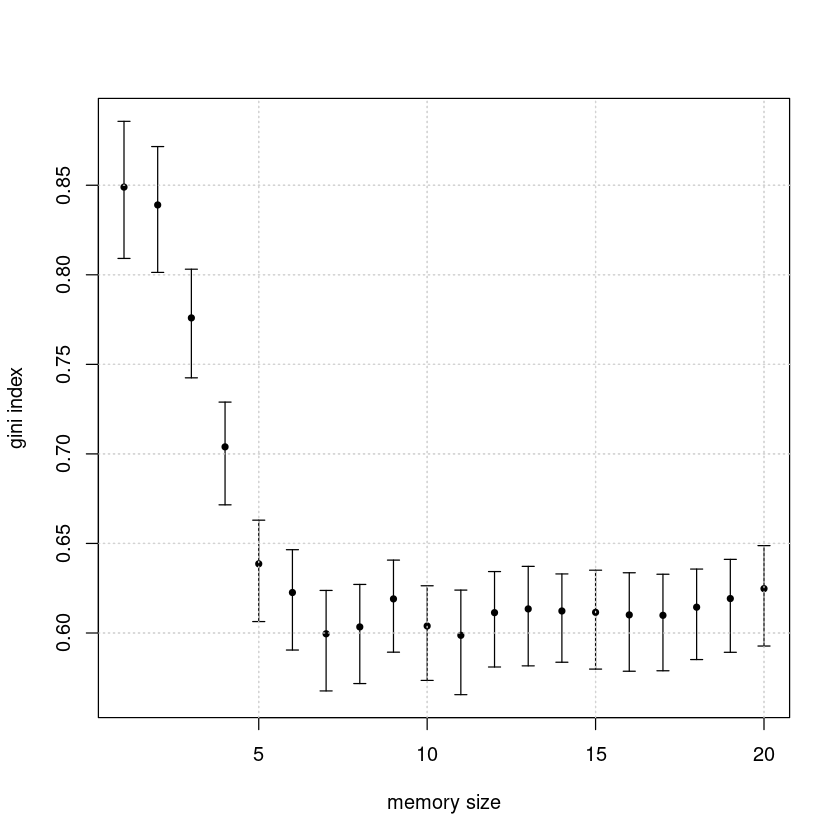
\includegraphics[width=.7\columnwidth]{img/gini_memory.png}
  %\caption{Gini index-memory plot with errorbars}
  %\label{fig:ginimem}
%\end{figure}
%
\begin{figure}[h]
  \centering
  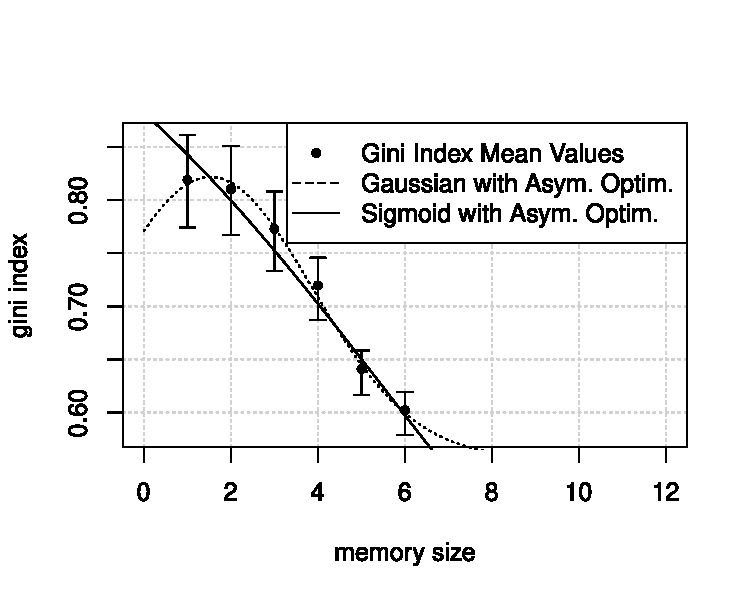
\includegraphics[trim={0cm 0cm 0cm 1cm},clip,width=.8\columnwidth]{img/gini.pdf}
  \caption[Gini index on memory size]
  {Gini index of fraction of users reached on memory size
    fitted with Gaussian and Sigmoid.
  }
  \label{fig:gini}
\end{figure}
%
\begin{table}[h]
  \centering
  \begin{tabular}{lcccc}
    \toprule
    & \multicolumn{2}{c}{\textit{Gaussian Fit}} & \multicolumn{2}{c}{\textit{Sigmoid Fit}}\\
     & {$\chi^2$} & {p-value} & {$\chi^2$} & {p-value} \\ \midrule
    \textit{std. err.} & \SI{1.3e-3}{} & \SI{9.7e-1}{} & \SI{8.1e-4}{} & \SI{9.8e-1}{} \\
    %\midrule[0.01em]
    \cmidrule(lr{0.01em}){2-5}
    \textit{quant. err.} & \SI{3.7e-3}{} & \SI{9.5e-1}{} & \SI{1.3e-3}{}  & \SI{9.7e-1}{} \\
    \textit{asym. err.} & \SI{1.4e-3}{} & \SI{9.7e-1}{} & \SI{8.4e-4}{} & \SI{9.8e-1}{} \\ \bottomrule
  \end{tabular}
  \caption[Reduced $\chi^2$ and p-value for Gaussian and Sigmoid fit]
  {Reduced $\chi^2$ and respective p-value for Gaussian
    and Sigmoid fit with different non-linear optimization
    strategies.\\
    Optimization using the standard error of the Gini index
    is denoted as std, quantile bootstrap optimization\cite{quantile} as
    quant and asymmetric error bar fitting optimization as asym.}
  \label{tab:gini}
\end{table}
%
We observe, sigmoid's $\chi^2$ is slightly lower than gaussian one,
for every error; p-value is higher instead.
Null hypothesis, for both measures, is far from being rejected:
goodness-of-fit is solidly validated.
Furthermore, sigmoid function would suggest a phase transition
in news' distribution. This behaviour is not new in network science:
the presence of a giant component
\footnote{A giant component is defined as a connected component
  of a random graph that contains a finite fraction of
  nodes\cite{giantwiki, giantbar}.}
in random graphs exhibits a sharp dependence from average degree
$\langle k \rangle$
\footnote{There are three regimes: subcritical
($\langle k \rangle <1$), supercritical ($\langle k \rangle >1$),
and connected ($\langle k \rangle >> ln(N)$,
N the total number of nodes).}.
If we start from zero and gradually increase value of
$\langle k \rangle$, giant component arises at the critical
point $\langle k \rangle =1$.
In kind, memory length could select different regimes
for news' distribution, although further studies would be necessary.
For these reasons, Sigmoid is our best-fit function for Gini
index-memory length plot.
